%%%%%%%%%%%%%%%
% Related Work and Background %
%%%%%%%%%%%%%%%

\section{Typology of Urban Forms}
To best understand the concept of road network patterns, one has to consider the urban forms of cities that best shape the road network patterns within such cities. Based on the literature on historic and more recent urban forms (for example, de Klerk, 1980; Rottier, 1980), identified six different forms (figure 2.1).
\begin{figure}[h]
\centering
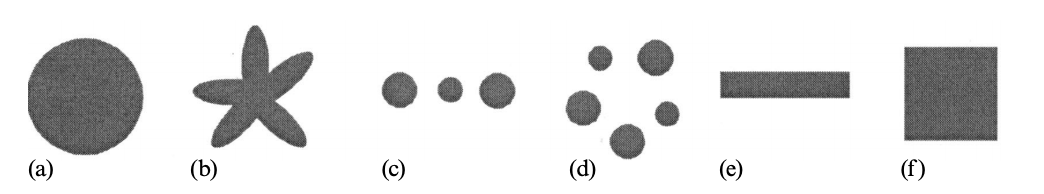
\includegraphics[width=0.95\textwidth,center]{picture/figure1.png}
\caption[Miniaturtrichter]{Morphological urban forms: (a) the concentric city, (b) the lobe city, (c) the linear polynuclear city, (d) the concentric polynuclear city, (e) the linear city, (f) and the grid city.  Source: de Klerk, 1980 \& Rottier, 1980}
\label{fig:urban forms}
\end{figure}

The concentric city represents the typical form of a city that has grown from a small (historic) center along a number of radial exit roads. Over the years the areas between the radial roads have been filled and the city has received its concentric form. This city shape is often associated with a radial road network, based on the historic routes, but combinations with ring or grid networks also exist. Often these cities are quite compact and have a strong center with a mixed supply of facilities.

The lobe city often has a similar history. The main differences are that the city has developed between some radial roads and not between others. The lobe shape can result from roads stretching out in some directions or from intentional city planning.

The linear polynuclear and concentric polynuclear cities have a number of things in common. The morphologies of these cities can develop in two very different ways. Either a number of smaller settlements, located close to each other, start to function as one city, or a city is actually designed as a polynuclear city. The only example of a true polynuclear city in the Netherlands is Almere, which can best be described as a concentric polynuclear city. 

The linear city can be viewed as an extreme version of the city form. These cities often have a grid-type transportation network for the car, but this is not necessarily the case. 

Grid cities is the collective noun for cities with a more or less rectangular shape. In the selection of locations for data collection these four types (concentric city, lobe city, and grid city) were included.


\section{Road network patterns}
The complexities of shape and structure set road patterns apart from many other objects of urban or transport analysis. For example, road width is merely a linear quantity and traffic flow is a simple ratio (vehicles per hour). Even the issue of density boils down to a straightforward ratio, however fiercely the significance of different numerators or denominators may be contested. By contrast, there is no straightforward or standard descriptor that is used to capture road patterns. 

Yet, unless we have an adequate description of pattern or structure, it will remain difficult to compare structures across cases – identifying patterns that are ‘good’ or ‘bad’ for different purposes – and hence make robust, generalisable recommendations for the design of urban layout.

Several approaches are used in the literature to classify the road pattern in an urban area. One common approach is based on the concept of macroscopic and microscopic street networks developed by Marshall (2005). The Macro-level or Citywide Street network distinguishes streets that are generally continuous over a substantial portion of the city and probably service travel from one part of the city to another and, in many cases, trips to or from the city. The Micro-level or Neighborhood Street network generally serves residential neighborhood travel because these streets are on routes that are not continuous over a significant portion of the city. Marshall (2005) then combines the four types of Citywide Street network types (linear, tributary, radial, and grid) with the two types of Neighbourhood Street network (tree and grid) to describe the street hierarchy in a city (Marshall & Garrick, 2010, 2011). 

Another common approach focuses directly on the overall street pattern in a community instead of focusing on the different types of streets and then combining the different types of streets to form a pattern. For example, Southworth \& Ben- Joseph (2003) classified street patterns into five categories: gridiron, fragmented parallel, wrapped parallel, loops and lollipops, and lollipops on a stick. Their classification is shown in Figure 2.2.

\begin{figure}[h]
\centering
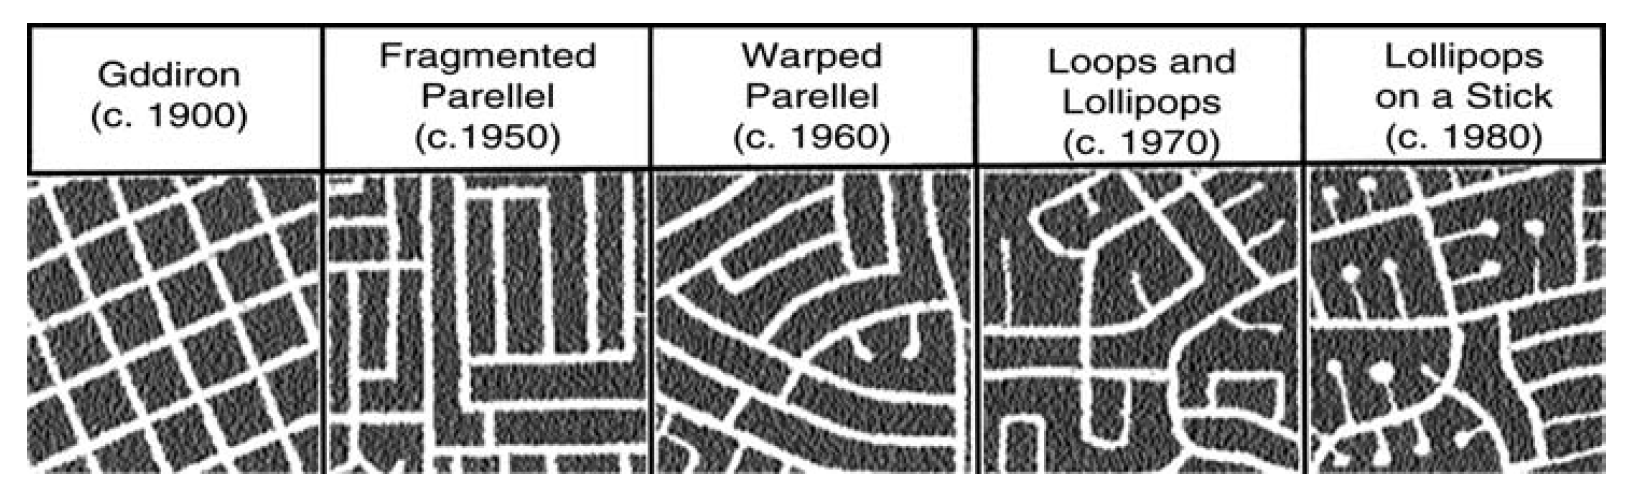
\includegraphics[width=0.95\textwidth,center]{picture/figure2.png}
\caption[Miniaturtrichter]{Types of street patterns. Source: Southworth \& Ben-Joseph (2003)}
\label{fig:streetpatterns}
\end{figure}

One major influencing factor to road network patterns is the typology (form or pattern) of the city themselves. To identify different road network types, Snellen, Borgers \& Timmermans (2002) study on the urban form, road network type, and mode choice for frequently conducted activities in the Netherlands is very useful. They distinguished between six principle urban forms, the concentric city, the lobe city, the linear polynuclear city, the concentric polynuclear city, the linear city, and the grid city as defined by de Klerk, 1980 \& Rottier, 1980. On the basis of these six principles, they identified five elementary networks. Their classification is shown in Figure 2.33. Since this approach forms the one of the basis for the classification scheme adopted in this study, a brief description of each will be presented.

The radial network is suitable for all transportation modes. For example, in the Netherlands, it is the classic network for urban public transport, where buses radiate to and from the city center or railway station. When used as a network for the other transport modes, it offers direct accessibility to the city center. However, this network type is also prone to congestion problems. In theory, it can be applied to all morphological urban forms. Snellen, Borgers \& Timmermans (2002).

\begin{figure}[h]
\centering
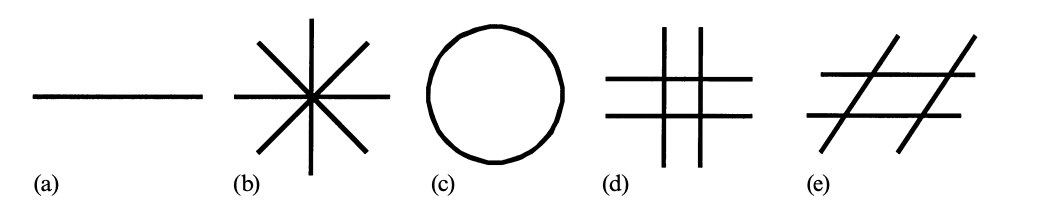
\includegraphics[width=0.95\textwidth,center]{picture/figure3.png}
\caption[Miniaturtrichter]{Figure 3. Elementary transportation networks: (a) the linear network, (b) the radial network, (c) the ring, (d) the grid, and (e) the shifted grid.  Source: Snellen, Borgers \& Timmermans (2002)}
\label{fig:transportnetworks}
\end{figure}

The ring network is frequently used mainly as a network for motorized transport. It offers the opportunity to concentrate a large amount of traffic on a single road, while other areas are relieved of traffic nuisance. In particular, city centers are often enclosed by a ring structure. This network type is not common for public transport in medium-sized cities, although it would provide good connections between city districts while avoiding a trip to and from the city center. For motorized and non motorized transport this network type can be applied to all morphological urban forms. For public transport, this network type is especially suitable for concentric polynuclear cities. Snellen, Borgers \& Timmermans (2002)

The (shifted) grid network is simple and direct, offers many choices of routes, and disperses traffic over many streets. Disadvantages of this network type are the many road crossings in the system. It is used mainly for motorized and non motorized transport. In theory, this network type is flexible and can be applied to all morphological urban forms. Snellen, Borgers \& Timmermans (2002)

[Chan, S.H.Y.; Donner, R.V.; L.mmer, S. Urban road networks-spatial networks with universal geometric features? Eur. Phys. J. B 2011, 84, 563–578.] divided a specific road network into four basic street network styles in their research, depicted in Figure 2.4 [Lima, M. The Book of Trees: Visualizing Branches of Knowledge; China Machine Press: Beijing, China, 2015; pp. 5–9. ISBN 978-7-111-51518-0.].  The patterns observed in their results are often observed in cities and conform to the real-world design requirements of a street network. Their approach serves as one of the foundations for the classification scheme used in this study, and each will be briefly described below.

\begin{figure}[h]
\centering
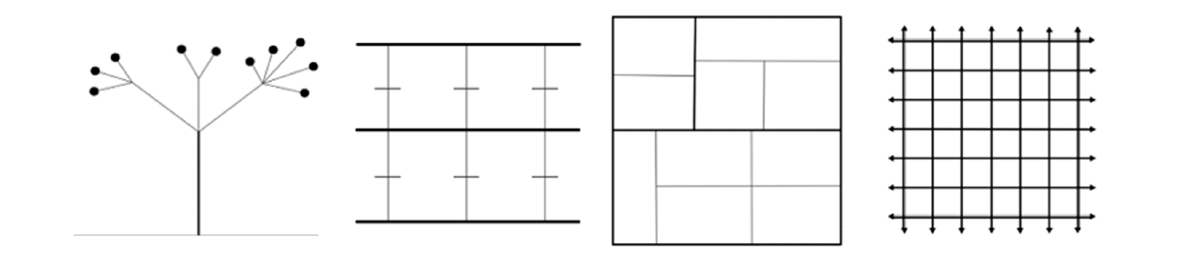
\includegraphics[width=0.95\textwidth,center]{picture/figure4.png}
\caption[Miniaturtrichter]{Abstract structures of four kinds of urban street networks. Source: Classification of Urban Street Networks Based on Tree-Like Network Features Baorui Han 1 , Dazhi Sun 2,*, Xiaomei Yu 1, Wanlu Song 1 and Lisha Ding 1)}
\label{fig:transportnetworks}
\end{figure}

Pure tree-like network pattern (Figure 2.4a). There are apparent backbone roads throughout the region and T-type cross and end-roads, forming a low-connected level network structure. This type of street network helps to protect residents' privacy and traffic stability, but it may be less robust than others.

The cul-de-sacs network pattern (Figure 2.4b). There are several trunks that run through a region with numerous end-roads. This type of network has good accessibility, but may be weaker in terms of interior connectivity than others.

T-type network pattern (Figure 4c). While this street network is similar to a pure grid-shaped network, the T-type intersections may improve trunk transportation efficiency while potentially reducing connectivity.

Pure grid-like network pattern (Figure 4d). Although this network is more connected than the others, transportation efficiency is typically lower due to the high number of intersections and short distances between them.

\section{Graph Networks}
A network is, in its simplest form, a collection of points joined together in pairs by lines. (Newman, 2010) "Network data structures for geographic information science (GIS) are methods for storing network data sets in a computer in order to support a range of network analysis procedures"[16 curtain]. A network can represent a transportation or communications system, a utility service mechanism, or a computer system, to name only a few network applications" [16]. Types of networks include flow networks and pure networks. Fischer explains flow networks will contain information on the flow of something within a network and a pure network represents any network's overall structure where the main concern are the topological relationships [17]. Additional examples of networks include computer networks, social networks, transport networks etc. Critical is the idea that a network by definition can be used to model and analyze linear features and their relationships. 

Networks, network models and network analysis are built upon the foundation of mathematics, typology and graph theory. Important contributions from graph theory are discussed in the next section and provide the foundation for characterizing networks, network analysis, and network pattern analysis.

A graph is an abstract representation of a set of elements and the connections between them (Trudeau, 1994). A graph consists of the following objects G = (N,E). In this example, G is the graph and the element N is interchangeably called the nodes (points) or vertices, and the connections between them E are called the edges (lines) or links. For consistency, this study uses the terms nodes and edges. The number of nodes in the graph (called the degree of the graph) is commonly represented as n and the number of edges as m. Two nodes are adjacent if an edge connects them, two edges are adjacent if they share the same node, and a node and an edge is incident, if the edge connects the node to another node. A model such as this is often depicted in the form of a picture. Figure 2.5, provides an example of a simple graph where there are three vertices and three edges. As a principle, vertices do not loop back upon themselves[19]. 

\begin{figure}[h]
\centering
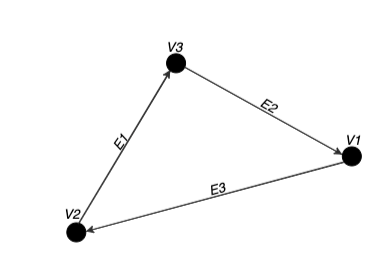
\includegraphics[width=0.95\textwidth,center]{picture/figure5.png}
\caption[Miniaturtrichter]{Directed Graph}
\label{fig:directedgraph}
\end{figure}

An undirected graph's edges point mutually in both directions, but a directed graph, or digraph, has directed edges (i.e., edge E2 points from node V3 to node V1, but there is not necessarily a reciprocal edge V3,V1). A self-loop is an edge that connects a single node to itself. Graphs can also have parallel (i.e., multiple) edges between the same two nodes. Such graphs are called multigraphs, or multi digraphs if they are directed. An undirected graph is connected if each of its nodes can be reached from any other node. A digraph is weakly connected if the undirected representation of the graph is connected, and strongly connected if each of its nodes can be reached from any other node. A path is an ordered sequence of edges that connects some ordered sequence of nodes. Two paths are internally node-disjoint if they have no nodes in common, besides end points. A weighted graph's edges have a weight attribute to quantify some value, such as importance or impedance, between connected nodes. The distance between two nodes is the number of edges in the path between them, while the weighted distance is the sum of the weight attributes of the edges in the path. (Boeing, 2017)

Leonhard Euler published the first noted example of problem solving using graph theory in 1736. He used a graph in his seminal paper to solve the Königsber Bridge Problem. He sought a solution in his writings to the use of seven bridges linking two islands to the banks and each other. The problem was crossing each bridge once without doubling back. Interestingly, using graph theory, he showed that no solution to the problem existed[19]. 

Graph theory and its implementations have developed since the time of Euler. Today, network modeling tends to be based on the same underlying concepts used by Euler, but the amount of knowledge that can be modeled and the complexity of the networks have expanded with the introduction of computers and GIS. Familiar examples include social networks (where individuals are the nodes and their interpersonal connections are the edges) and the World Wide Web (where web pages are the nodes and hyperlinks leading from one to another are the edges). A complex network (the configuration and arrangement of its nodes and edges) is one with a non-trivial topology, i.e. the topology is neither entirely regular nor totally random. The majority of big real-world networks (Newman, 2010) are dynamic. Complex spatial networks, i.e. complex networks with nodes and/or edges embedded in space, are of special importance in this analysis (O'Sullivan, 2014). A street network, as well as railways, power grids, and water and sanitation networks, is an example of a dynamic spatial network of both nodes and edges embedded in space (Barthélemy, 2011). Newman 's 2003 paper, "The Structure and Role of Complex Networks," is recommended for more in-depth review[6].

\section{Road network as Graphs}
Road networks are usually modeled as graphs, with nodes representing intersections and dead ends, and edges representing street segments connecting them (Barthelemy and Flammini, 2008; Cardillo et al., 2006; Lin and Ban, 2013; Marshall et al . , 2018; Porta et al., 2006). These edges are embedded in space and have a bearing of both length and compass (Barthelemy, 2011). The current research models urban street networks with potential  self-loops as undirected nonplanar multigraphs. Though most-faithfully guided graphs reflect flow restrictions (such as vehicular traffic on one-way roads), undirected graphs best model urban structure by referring to street segments (i.e. the linear sides of city blocks) by 1:1. Although many street networks are roughly planar (with very few overpasses or underpasses), by accommodating certain bridges and tunnels which also occur, nonplanar graphs offer more detailed models (Boeing, 2018c; Eppstein and Goodrich, 2008).

Data used to study these networks typically comes from the shapefiles of digitized streets. The data can be generated by individual local, state or federal entities within each country, but the criteria for digitization and availability of the data differ. As a result, cross-sectional street network orientation and entropy analysis tended to be confined to unique geographic areas or to analyze small samples (Boeing, 2019). Today, however, OpenStreetMap offers a new alternate data source. OpenStreetMap is a global collaborative mapping initiative comprising highways, houses, services, and other spatial features. Although the quality of its data varies somewhat across countries, its street data is generally of high quality,  especially in cities (Barrington-Leigh and Millard-Ball, 2017; Barron et al. , 2014; Zielstra et al., 2013). The OpenStreetMap data source gives the ability to conduct cross-sectional research into the form and layout of street networks around the world. Researchers have recently studied the order and disorder of the street network through the  circuity and orientation entropy. Circuity focuses on the measures of the street curvature and how it applies to other urban network patterns (Boeing, 2019; Giacomin and Levinson, 2015;  Levinson and El- Geneidy, 2009). The orientation entropy quantifies and visualizes the entropy of street orientations in order to determine how ordered they are (Courtat et al., 2011; Gudmundsson and Mohajeri, 2013; Mohajeri et al., 2013a, 2013b; Mohajeri and Gudmundsson, 2014, 2012). In their research, Louf and Barthelemy (2014) studied the geometry of city blocks around the world as a function of block size and form factor, clustering them together to define the differences between US and European cities. However, little is understood about cross-sectional patterns in the spatial orientation and ordering of road networks around the world. This thesis draws on this previous analysis into circuitry, order, and entropy by building on OpenStreetMap data to analyze cities around the world and investigate similarities in their patterns and relationships.

A spatial network is planar if it can be represented with its edges intersecting only at nodes in two dimensions. For example, a road network may be planar (especially in some small scales), but most road networks are non-planar due to grade-separated expressways, overpasses, bridges, and tunnels (Boeing, 2017). In spite of this, a large number of existing quantitative analyses of urban street networks represent them as planar graphs for tractability (Barthélemy & Flammini, 2008; Buhl et al., 2006; Cardillo, Scellato, Latora, & Porta, 2006; Masucci, Smith, Crooks, & Batty, 2009; Strano et al., 2013, since bridges and tunnels are comparatively rare (in some places), so the networks are roughly planar. However, this oversimplification of tractability planarity can be needless and may cause methodological problems. The street networks mentioned so far are known as primal graphs that represent nodes as intersections and edges as street segments. This thesis, however, focuses on primal graphs because they preserve all the geographical, spatial, and metric information essential to the urban form and design that dual representations discard for a  street network as all the such as the length, shape, circuity, width, etc. The primal graph, on the other hand, represents all the spatial characteristics of a street network. Using Primal graphs may be a better approach to analyzing spatial networks where geography matters, since the physical space underlying the networks themselves contains the relevant information that cannot exist in the topology of the network alone (Ratti, 2004).

\subsection{Evaluation Metrics of Road Networks}
Road network topology is defined as the spatial arrangement of roads at a given location (Rodrigue, Comtois, \& Slack, 2016). It is conventionally evaluated by the measures of gridness, treeness, ringness, webness, (Barthélemy, 2011; Buhl et al., 2006; Gudmundsson \& Mohajeri, 2013; Xie \& Levinson, 2007) and typology (Louf \& Barthelemy, 2014). Recent advances in topology, graph theories and the growth in computing ability has paved the way for more advanced methods for quantitative analysis of road network patterns (Bavelas, 1948; Jiang \& Claramunt, 2004; Cardillo, Scellato, Latora, \& Porta, 2006).

In their research, Xie \& Levinson, 2007 \& Levinson, 2012, pointed out that the two fundamental structures commonly observed in the planar transport network include the tree-like network and grid-like network. In this regard, Noda (1996) introduced the grid-tree-proportion index (GTP index) as a new mathematical measure uniting the alpha and gamma indices used to jointly evaluate the grid pattern, tree pattern, and other road network patterns that do not belong to either of the two categories  highlighted (Usui \& Asami, 2011). The approach is also used to quantify the formation, coherence and connectivity of road network patterns (Gogoi; Usui \& Asami, 2011; X. Wang, You, & Wang, 2017). In addition, it is used to assess the efficiency of traffic flow or movement in the road network. The GTP index ranges from the lowest value of 0 to the highest value of 1. The GTP index coefficient is computed by substituting the following formula.

\begin{equation}
{GTP}=\frac{e-V+1}{\left(\sqrt{V-1)^{2}}\right.}
\end{equation}

Where:
GTP $=$ Grid Tree Pattern
$\mathrm{e}=$ Total number of edges (Links)
$\mathrm{V}=$ Total number of vertex (Nodes)
\caption{Source: Tini \& Shah, 2018}

Road networks considered to be primal, non-planar, weighted multi-digraphs with self-loops can be characterized, described and evaluated by both metric and topological measures. Extended concepts and algorithms can be found in Newman (2010) and Barthélemy (2011). 

Measured in terms of length and area, the metric structure represents common transportation variables (Cervero \& Kockelman, 1997; Ewing \& Cervero, 2010). Boeing (2017), defined the following major metric measures for density as “average street length, mean edge length (in spatial units such as meters) in the undirected representation of the graph which all act as the linear proxy for block size and shows how fine-grained or coarse-grained the network is. Node density is the number of nodes divided by the area covered by the network. Intersection density is the node density of the group of nodes with more than one street emanating from them (excluding dead-ends). The edge density is the sum of all edge lengths divided by the area, and the physical street density is the sum of all edges in the undirected representation of the graph divided by the area”. All these density measures give a further indication of how fine-grained the network is. Finally, the average circuity divides the sum of all edge lengths by the sum of the great-circle distances between the nodes incident to each edge (cf. Giacomin \& Levinson, 2015). This is the average ratio between the length of the edge and the straight-line distance between the two nodes it connects.

Topological measures of the structure of a street network often indicate the configuration, connectedness, and robustness of the network as well as how these characteristics are distributed. The average node degree, or mean number of edges that are incident to each node, quantifies the connectivity of each node on average. “Similarly, but more precisely, the average streets per node measures the mean number of physical streets emanating from each intersection and dead-end. This adapts the average node degree to the physical form rather than to the directed circulation” Boeing (2017). The statistical and spatial distributions of the number of streets per intersection describe the type, prevalence, and dispersion of the connectivity of all intersections in the network. Connectivity measures the minimum number of nodes or edges to be removed from a connected graph in order to disconnect it. It is considered to be a measure of resilience, since complex networks with high connectivity offer more routing options for agents and are more robust to failure. However, node and edge connectivity is less effective for approximately planar networks like street networks: most street networks will have the connectivity of 1, because the presence of a single dead-end means the removal of just one node or edge can disconnect the network. More usefully, the average node connectivity of a network the mean number of internally node-disjoint paths between each pair of nodes within the graph represents the expected number of nodes that has to be removed to disconnect a randomly selected pair of non-adjacent nodes (Beineke, Oellermann, \& Pippert, 2002). As O'Sullivan (2014) explains, both spatial integration and approximate planarity greatly limits a network’s distance, degrees and connectivity. Other measures of connectedness within a network such as intersection density, node degree distribution, and centrality/clustering (discussed in the next paragraph) can better capture the nature of a street network's connectedness than node or edge connectivity. Low connectedness networks can have several single points of failure, making the system especially vulnerable to perturbation. This is evident in urban design by the way of permeability and choke points, for instance, traffic jams can occur and circulation networks can fail if circulation within the network is forced through single points of failure. (Hajrasouliha \& Yin, 2015) linked connectedness to pedestrian volume within a street network.

In addition to being able to better capture the nature of the connectedness of a road network than node or edge connectivity, clustering measures also show the topological structure and distribution of a street network. Boeing 2017, describes a node’s clustering coefficient as “the ratio of the number of edges between its neighbors to the maximum possible number of edges that would exist between these neighbors”. The weighted clustering coefficient is used to calculate the connectivity and complexity from how thoroughly the neighborhood of a given node is connected together, since it weighs the connectivity and complexity ratio from edge length and the average clustering coefficient as the mean of the clustering coefficients of all the nodes in the network. The weighted clustering coefficient was extended to neighborhoods within an arbitrary distance by Jiang and Claramunt (2004) to make it more applicable to urban street networks. The importance of nodes in a network is indicated by the Centrality. Barthélemy, 2004, describes the Betweenness centrality as the evaluation of the number of shortest paths that pass through each node or edge. The maximum betweenness centrality in a network specifies the  proportion of shortest paths that pass through the most important node/edge. This is a measure of resilience: networks with a high maximum betweenness centrality are more vulnerable to failure if the single choke point fails. The average betweenness centrality is the mean of all the betweenness centralities in the network (Barthélemy, 2011). In their work, Barthélemy, Bordin, Berestycki, and Gribaudi (2013) used the betweenness centrality to identify top-down interventions against the bottom-up self-organization and evolution of Paris's urban network pattern. Closeness centrality represents, for each node, a reciprocal sum of the distance from that node to all other nodes in the network: that is, nodes rank as more central if they are on average similar to all other nodes. Finally, PageRank, developed by Brin & Page, 1998 is the algorithm used by Google to rank web pages. The PageRank algorithm is known to be a variant of the network centrality, namely the eigenvector centrality. PageRank can also be extended to street networks, as it ranks nodes on the basis of the structure of incoming links and the rank of the source node. (Agryzkov, Oliver, Tortosa, \& Vicent, 2012; Chin &Wen, 2015).


\section{Graph Similarity Measures}
Comparing Graph Similarity Measures for Semantic Representations of Documents Rub´en Manrique(B) , Felipe Cueto-Ramirez , and Olga Mari˜no Systems and Computing Engineering Department, School of Engineering, Universidad de los Andes, Bogot´a, Colombia {rf.manrique,f.cueto10,olmarino}@uniandes.edu.co

As a result of the recent developments on graph matching, different algorithms have been proposed to solve the problem of comparing graph-based representation [Bunke, H.: Recent developments in graph matching. In: Proceedings 15th International Conference on Pattern Recognition, ICPR-2000, vol. 2, pp. 117–124 (2000)]. Though little has been explored in this regard for road network representations, these graph matching algorithms can be adapted in order to support the calculation of similarities. Some of the most important measures are presented in the following paragraphs. It is also important to emphasize that there is not a single criterion to choose the best measure since their performance does greatly depend on the characteristics of the graph [16]. As such, experimentation is the most appropriate way to select the best algorithm for the problem at hand [Jouili, S., Tabbone, S., Valveny, E.: Comparing graph similarity measures for graphical recognition. In: Ogier, J.-M., Liu, W., Llad´os, J. (eds.) GREC 2009. LNCS, vol. 6020, pp. 37–48. Springer, Heidelberg (2010). https://doi.org/10.1007/ 978-3-642-13728-0 4]. 

These following descriptions below aren't comprehensive descriptions of every graph comparison method in use today, but they do show some similarities between them.

\subsection{Graph Edit Distance / Graph Isomorphism}
Graph isomorphism is one method for evaluating graph similarity. If two graphs are isomorphic, they are similar [M Pelillo. Replicator equations, maximal cliques, and graph isomorphism. Neural Computation, 11(8):1933–1955, 1999.], or one is isomorphic to a subgraph of the other , or they contain isomorphic subgraphs. The disadvantage of graph isomorphism is that the exact versions of the algorithms are exponential making them inapplicable to today's large graphs.  The graph edit distance is a variant of the graph isomorphism problem, in which the goal is to transform one graph into another by performing a series of operations (additions, deletions, substitutions of nodes or edges, and reversions of edges). This method assigns a cost to each operation and seeks to find the operation sequence that will minimize the cost of matching the two graphs.[Algorithms for Graph Similarity and Subgraph Matching, Danai Koutra et  al 2011]

GED (graph edit distance) is a more flexible similarity measure that contemplates the differences in edges and nodes as well as the set of associated weights [Gao, X., Xiao, B., Tao, D., Li, X.: A survey of graph edit distance. Pattern Anal. Appl. 13(1), 113–129 (2010)]. There are many adaptations of GED; however, the use of the bipartite variation of GED [4] to limit algorithm complexity has been used as much as possible (Comparing Graph Similarity Measures for Semantic Representations of Documents Rub´en Manrique(B) , Felipe Cueto-Ramirez , and Olga Mari˜no ). 

The most basic graph distances and extensions aggregate element-by-element comparisons between the adjacency matrices of two graphs; [Golub G, van Loan C. 2013Matrix computations. Baltimore, MD: JHU Press. 1421407949 9781421407944,  Jaccard P. 1901Étude de la distribution florale dans une portion des Alpes et du Jura. Bull. de la Societe Vaudoise des Sciences Naturelles 37, 547–579. (doi:10.5169/seals-266450),  Hamming RW. 1950Error detecting and error correcting codes. Bell Syst. Tech. J. 29, 147–160. (doi:10.1016/S0016-0032(23)90506-5),  Gao X, Xiao B, Tao D, Li X. 2010A survey of graph edit distance. Pattern Anal. Appl. 13, 113–129. (doi:10.1109/GlobalSIP.2013.6736904)][Wallis W, Shoubridge P, Kraetz M, Ray D. 2001Graph distances using graph union. Pattern Recognit. Lett. 22, 701–704. (doi:10.1016/S0167-8655(01)00022-8)]; because these methods are known to explicitly depend on the node labeling scheme (and are therefore not invariant under graph isomorphism [Chowdhury S, Mémoli F. 2017Distances and isomorphism between networks and the stability of network invariants.]), their utility when comparing graphs with unknown labels  may be limited (e.g. graphs sampled from random graph ensembles). Several measures collect empirical distributions [Carpi L, Rosso O, Saco P, Ravetti M. 2011Analyzing complex networks evolution through information theory quantifiers. Phys. Lett. A 375, 801–804. (doi:10.1016/j.physleta.2010.12.038)] or a “signature” vector [Berlingerio M, Koutra D, Eliassi-Rad T, Faloutsos C. 2012NetSimile: a scalable approach to size-independent network similarity.] from each graph and compute the distance between them (using the Jensen-Shannon divergence, Canberra distance, earth mover’s distance, and other measures. [Emmert-Streib F, Dehmer M, Shi Y. 2016Fifty years of graph matching, network alignment and network comparison. Inf. Sci. 346, 180–197. (doi:10.1016/j.ins.2016.01.074)]), which allows for the comparison of graphs with different sizes. [Bagrow J, Bollt E. 2019An information-theoretic, all-scales approach to comparing networks. Appl. Netw. Sci. 45, 1–15. (doi:10.1007/s41109-019-0156-x), Meilǎ M. 2007Comparing clusterings-an information based distance. J. Multivariate Anal. 98, 873–895. (doi:10.1016/j.jmva.2006.11.013)].

\subsection{Signature Similarity}
Signature similarity [Papadimitriou, P., Dasdan, A., Garcia-Molina, H.: Web graph similarity for anomaly detection. J. Internet Serv. Appl. 1(1), 19–30 (2010) ] is another graph similarity metric to consider. Using the node weights, the method attempts to generate a signature vector of 1s and 0s for each graph. The vectors are then compared by counting the number of matches between them. It normalizes the result and provides similarity measurements between 0 and 1.

\subsection{Spectral Distance}
Another approach is comparing the spectral properties of certain matrices characterized by graphs [Jurman G, Visintainer R, Filosi M, Riccadonna S, Furlanello C. 2015The HIM glocal metric and kernel for network comparison and classification. In Proc. of the 2015 IEEE Int. Conf. on Data Science and Advanced Analytics, DSAA. 1–10. (doi:10.1109/DSAA.2015.7344816)], such as the non-backtracking matrix [Torres L, Suárez-Serrato P, Eliassi-Rad T. 2019Non-backtracking cycles: Length spectrum theory and graph mining applications. Appl. Netw. Sci. 4, 41 (doi:10.1007/s41109-019-0147-y), Mellor A, Grusovin A. 2019Graph comparison via the nonbacktracking spectrum. Phys. Rev. E 99, 052309.] or Laplacian matrix [Jurman G, Visintainer R, Furlanello C. 2011An introduction to spectral distances in networks. Neural Nets WIRN10: Proceedings of the 20th Italian Workshop on Neural Nets. 227–234. (doi:10.3233/978-1-60750-692-8-227)], which is known as spectral distance. The relevant spectral properties associated with these distances are invariant under graph isomorphism. [Chowdhury S, Mémoli F. 2017Distances and isomorphism between networks and the stability of network invariants. (http://arxiv.org/abs/1708.04727), van Steen M. 2010Graph theory and complex networks. An Introduction. Amsterdam, The Netherlands: Maarten van Steen. 978-90-815406-1-2.]. Some of these graph distance measures have been proven to be metrics (that is, they satisfy properties like triangle inequality, etc.) [Deza MM, Deza E. 2009Encyclopedia of distances. New York, NY: Springer(esp. Section 1.1, pp. 3–10).], while others have not.

\subsection{Feature-based Distance}
Looking at specific "features" of the graph, such as the degree distribution, betweenness centrality distribution, diameter, number of triangles, number of k-cliques, and so on, is one method for comparing graphs. For vector-valued graph features (such as degree distribution), one could also consider the vector as an empirical distribution and use the sample moments as graph features (or quantiles, or statistical properties). A feature-based distance is one that compares graphs by comparing such features.

Of course, all of the methods discussed thus far are feature-based in general; however, in the special case where the features occur as values over the space V V of possible node pairings, they are often referred to as  matrix distances. Similarly, if the feature in question is the spectrum of a specific matrix realization of the graph, the method is referred to as a spectral distance.

[Berlingerio M, Koutra D, Eliassi-Rad T, Faloutsos C. NetSimile: A Scalable Approach to Size-Independent Network Similarity. CoRR. 2012;abs/1209.2684. ] proposes NETSIMILE, which is a feature-based distance with the  focus on local and egonet-based features (e.g., degree, volume of egonet as fraction of maximum possible volume, etc.). When k features are used, the method generates a feature-vertex matrix of size k n. The associated feature matrix generated is then reduced to a "signature vector" (a process referred to as "aggregation" by the authors of [Berlingerio M, Koutra D, Eliassi-Rad T, Faloutsos C. NetSimile: A Scalable Approach to Size-Independent Network Similarity. CoRR. 2012;abs/1209.2684.] that consists of the mean, median, standard deviation, skewness, and kurtosis of each These signature vectors are then compared to determine the distance between graphs.

Feature-based methods for comparing graphs are popular in the neuroscience literature, in particular [Bassett DS, Bullmore E, Verchinski BA, Mattay VS, Weinberger DR, Meyer-Lindenberg A. Hierarchical organization of human cortical networks in health and schizophrenia. Journal of Neuroscience. 2008; 28(37):9239–9248. https://doi.org/10.1523/JNEUROSCI.1929-08.2008 PMID: 18784304 , Kaiser M. A tutorial in connectome analysis: topological and spatial features of brain networks. Neuroimage. 2011; 57(3):892–907. https://doi.org/10.1016/j.neuroimage.2011.05.025 PMID: 21605688 ]. The authors [van den Heuvel MP, Sporns O, Collin G, Scheewe T, Mandl RCW, Cahn W, et al. Abnormal rich club organization and functional brain dynamics in schizophrenia. JAMA Psychiatry. 2013; 70(8):783–792.] compared the functional connectivity networks of patients with and without schizophrenia using graph features such as modularity, shortest path distance, clustering coefficient, and global efficiency. Using standard statistical techniques, the statistics for these features for the control and experiment groups are aggregated and compared.

\subsection{Maximum Common Subgraph}
A different approach to graph similarity is the Maximum Common Subgraph. Different variations that have been proposed for the MCS (Maximum common subgraph) algorithm [Bunke, H., Shearer, K.: A graph distance metric based on the maximal common subgraph. Pattern Recognit. Lett. 19(3), 255–259 (1998) ]. The MCS is the largest subgraph that is common in the considered graphs. Different metrics use the size of the MCS as an indicative of similarity. The size of a sub-graph can be measured in several ways, but the focus of this thesis will be on the number of nodes. This method is especially useful in biological and chemical analysis [willet], as well as the graph kernel approach. Chapter 3 goes into greater detail about its application.

\subsection{Vertex Edge Overlap}
VEO (vertex edge overlap) [ Papadimitriou, P., Dasdan, A., Garcia-Molina, H.: Web graph similarity for anomaly detection. J. Internet Serv. Appl. 1(1), 19–30 (2010), Comparing Graph Similarity Measures for Semantic Representations of Documents Rub´en Manrique(B) , Felipe Cueto-Ramirez , and Olga Mari˜no ] is a basic strategy that measures the similarity between two graphs by calculating the overlap between their edges and nodes, ignoring the edge or node weights.  This method  attempts to simplify the graph matching problem by counting the total number of vertices and edges that match and dividing the result by the sum of the total number of vertices and edges on each graph. This factor is multiplied by 2 in order to normalize the result appropriately.[Comparing Graph Similarity Measures for Semantic Representations of Documents Rub´en Manrique(B) , Felipe Cueto-Ramirez , and Olga Mari˜no]

\begin{equation}
V E O\left(G, G^{\prime}\right)=2 \frac{\left|V \cap V^{\prime}\right|+\left|E \cap E^{\prime}\right|}{|V|+\left|V^{\prime}\right|+|E|+\left|E^{\prime}\right|}
\end{equation}

Because it only uses variables from the graph, this algorithm can be applied to any graph structure. Even so, it is an extremely limited approach because it does not take into account information such as vertex or edge weight or path information. This method is based on a simplified version of the GED (Graph edit distance) algorithm and is normalized to a scale of 1 to 0, with 1 being completely similar and 0 being completely dissimilar. The complexity of this algorithm is O(V + E) because it only requires a single iteration over the sets of one of the graphs to find the matching pairs in both vertices and edges.


\subsection{Graph Clustering}
The term Graph clustering is currently used in literature for two distinct and unrelated interpretations, each of which may be of concern to researchers working in the field of Pattern Recognition: in the first sense, graphs are used to represent each of the items to be clustered, so clustering is done on a collection of graphs. In the second sense, which is the most commonly found, according to P.Foggia et al, 2014 “a single graph is used to represent the structure of the space to which the objects belong with a node for every object and edges encoding the relationships between pairs of objects usually a similarity or a distance measure is related to each edge; in this case, the clustering is carried out by splitting the set of nodes of the graph according to some criterion”. Of particular interest to this study is the clustering of graphs which is used to find the similarity between different road network patterns represented as graphs.

\subsection{Clustering of Graphs}
For the clustering of graphs, (Gunter and Bunke, 2002) proposed an application to graphs with the Unsupervised Learning Vector Quantization (LVQ) algorithm. The algorithm uses Graph Edit Distance to determine the distance between an input graph and a prototype cluster and an initial GED-based algorithm that determines the weighted combination of two graphs (by calculating the minimum number of editing operations to transform the first graph to the second, and then by choosing a subset of these operations depending on the weight), which is used for updating the winning prototype. The same authors suggested an extension of this approach in 2003 (Gunter and Bunke, 2003), adding a series of validity indices for clustering to pick the optimum number of LVQ nodes. (Serratosa et al.2002) proposed an algorithm based on Function-Described Graphs for the clustering of graphs, which are Attributed Relational Graphs, extended with information about the node and edge joint probability constraints. The algorithm is based on an incremental, hierarchical clustering strategy. (Jain and Obermayer, 2011) in their paper presented a method for the clustering of graphs based on the Vector Quantization with the k-Means algorithm. To perform the quantization, the suggested algorithm uses the integration of graphs into Riemannian orbit folds, based on Graph Edit Distance. The authors explored in-depth the theoretical characteristics of the proposed solution, pointing out some necessary conditions for the optimality of the clustering found and for statistical consistency; the authors also discussed the effect of potential approximations on reducing the cost of computing.

\begin{figure}[h]
\centering
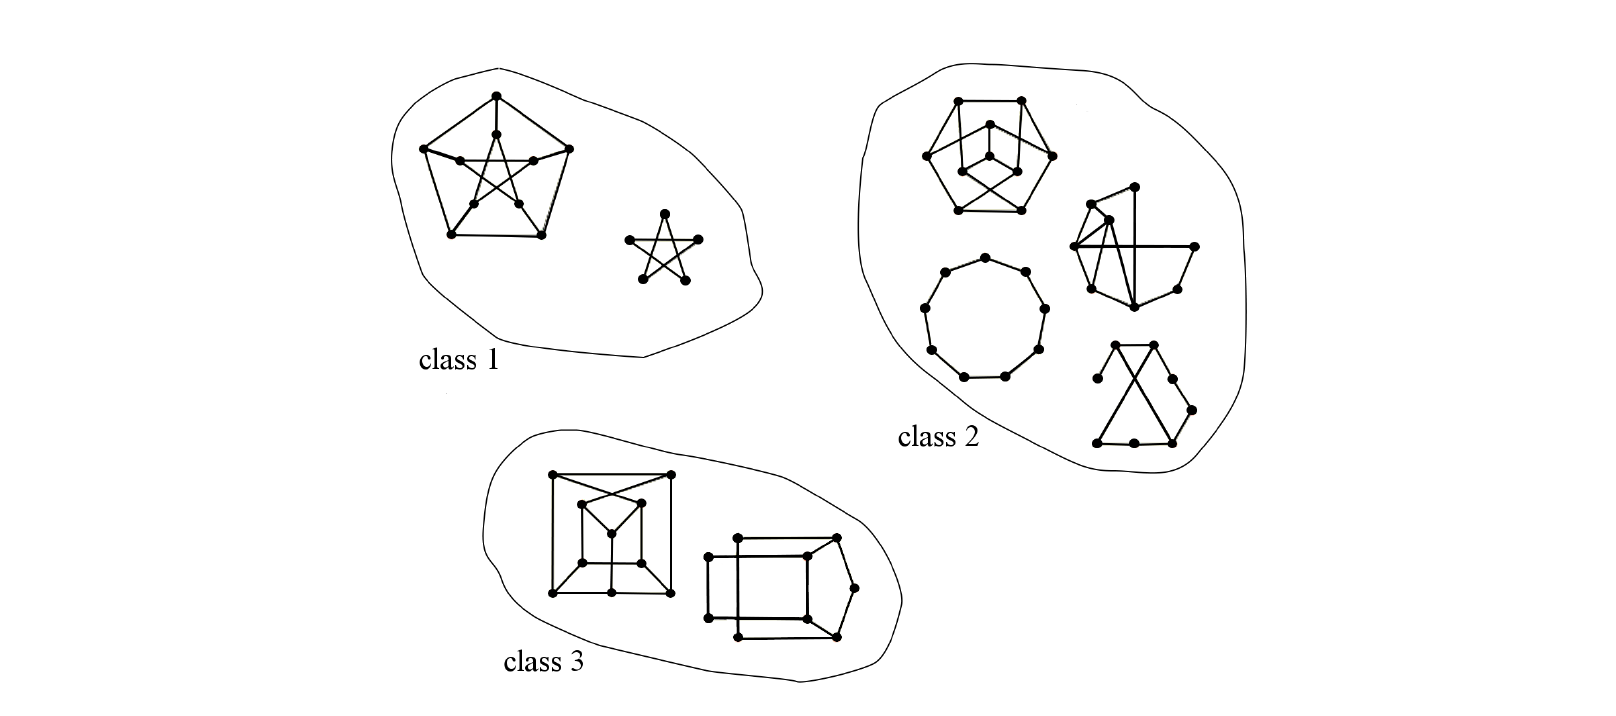
\includegraphics[width=0.95\textwidth,center]{picture/figure6.png}
\caption[Miniaturtrichter]{Clustering of graphs: each of the objects to be clustered is represented by a graph. Source: P.Foggia, G.Percannella and M.Vento, 2014}
\label{fig:clusteringgraphs}
\end{figure}


\subsection{Graph Kernels}
A graph kernel is a function that maps a few graphs to a real number, and has similar properties to the vector-defined dot product. More formally, if we denote the space of all the graphs with G, a graph kernel is a function k such as:

\begin{equation}
k: \mathbb{G} \times \mathbb{G} \longrightarrow \mathbb{R}
\end{equation}
\begin{equation}
k\left(G_{1}, G_{2}\right)=k\left(G_{2}, G_{1}\right) \quad \forall G_{1}, G_{2} \in \mathbb{G}
\end{equation}
\begin{equation}
\sum_{i=1}^{n} \sum_{j=1}^{n} c_{i} \cdot c_{j} \cdot k\left(G_{i}, G_{j}\right) \geq 0
\end{equation}
\begin{equation}
\forall G_{1}, \ldots, G_{2} \in \mathbb{G}, \forall c_{1}, \ldots, c_{n} \in \mathbb{R}
\end{equation}

In the equation 2.5.3 above, the function k is required to be symmetric, while Equation's 2.5.4 and 2.5.5 respectively requires it to be positive semi-definite. Source: P.Foggia, G.Percannella and M.Vento, 2014

A graph kernel can be viewed informally as a measure of the similarities between two graphs; however, its formal properties allow a kernel to replace a vector dot product with many vector-based algorithms (and other dot-related functions, such as the Euclidean standard) that use this operator. Thanks to the Mercer theorem, kernels have long been used to extend linear algorithms operating on vector spaces to nonlinear cases: given the kernel function defined on compact Hausdor space X, vector space V and mapping between X and V are used in such a way that the kernel value calculated on two points in X is equal to the dot product of the corresponding points in V. While the theorem of Mercer does not apply to graph kernels, the latter can be used in practice as a theoretically sound way to extend a vector algorithm to graphs. The efficiency of these algorithms, greatly depends on the appropriateness of the notion of similarity expressed within the graph kernel (with relevancy to the task at hand). (P.Foggia, G.Percannella and M.Vento, 2014)

(Kashima et al. 2003), in their paper, they proposed the idea of marginalized kernels, a probabilistic approach for defining a kernel based on the introduction of specialized hidden variables for the graph domain. In this case, the hidden variable is a sequence of node indices generated on one of the graphs according to a random walk. Provided the value of the concealed variable, the sequence kernel is calculated using the sequence of nodes and edges visited; the marginalized kernel is calculated by estimating the estimated value of the sequence kernel (concerning the combined distribution of the hidden and visible variables). (Mahe and Vert, 2009) extended this technique to trees and presented a molecular data application. To avoid the exponential cost of enumerating all the paths in a graph, the authors proposed a scheme to use only the shortest path between any pair of nodes since the shortest paths can be calculated in polynomial time. (Borgwardt and Kriegel, 2005) presented a graph kernel based on paths instead of walks (a path is a walk without repeated nodes). (Neuhaus and Bunke, 2006), introduced three graph kernels based on Graph Edit Distance in their paper. The first kernel requires a zero pattern to be chosen, a graph that will act similarly to a null vector with respect to the kernel. The authors found that the kernel fulfills the theoretical requirements of a kernel function, but it's functional performance is significantly influenced by the choice of the zero patterns. The authors then introduced two other kernels, obtained over a set of zero patterns from the sum and the product of the first kernel, and proved that they have the same theoretical properties but are more stable in choosing these patterns.

(Neuhaus et al , 2009) in their paper,  presented three possible ways to use Graph Edit Distance in the definition of a kernel. The first way is a diffusion kernel, which transforms the edit distance matrix into a positive definite matrix that satisfies the properties of the kernel, but has the inconvenience that the set of graphs on which it is applied must be finite and known a priori. The second way is a convolution kernel which is based on the decomposition of the edit path between the two graphs into a sequence of substitution operations; this method provides a definition for a kernel between two graphs, given the kernel for individual substitutions. The only downside is the exponential complexity of the number of nodes for which an estimate is proposed by the authors. A random walk kernel is the third way, where the Graph Edit Distance is used to denote a fuzzy graph of the product from which a kernel is obtained that evaluates the local similarity of the corresponding parts of the two graphs.

Gauzere et al. 's 2012 paper introduces two graph kernels. The first is based on the Graph Edit Distance, called the Laplacian Kernel. The operation of the product extracted from the Graph Edit Distance is not guaranteed to be positive definite, and thus does not have the formal properties of the kernel; thus, the authors recommended a technique to obtain a positive definite matrix from the distance matrix, which is then used as the kernel. The second kernel, known as the treelet kernel, is based on treelets, which are all potential trees with less than a fixed number of nodes (up to 6 nodes are considered in the papers); the kernel is determined by counting the occurrences of each treelet in the graphs. Only unattributed graphs can use this kernel, while the Laplacian kernel can also be used for graphs with node and edge attributes. The same authors also later suggested a kernel that is also based on treelets but uses a treelet edit distance instead of merely counting their occurrences to equate the treelets in one graph with those in the other, so as to be tolerant of minor deformations of the graphs. In their article, Grenier et al, 2013 suggested a different treelet-based kernel, especially developed for applications in chemoinformatics, which often integrates knowledge within the graph on the position of each treelet. 

B. Strug, 2011 proposes a kernel based on combining a tree kernel with a classical graph kernel, explicitly developed for hierarchical graphs.